\chapter{Resultaten}
De algoritmes worden getest in een on-line situatie gegenereerd door de simulatie. Er is enkel ruis toegevoegd op het koppel geleverd door de fietser. De modellen beginnen van nul. Gedurende een startperiode leren de algoritmes bij en zal de cadans bepaald worden door het fietsersmodel. Na de startperiode nemen de algoritmes deze instelling over. Na elke voorspelling wordt de mean squared error berekend tussen de voorspelling en het fietsersmodel. Elke 30 iteraties wordt er afgewogen of de algoritmes te ver afwijken van het fietsersmodel. Wanneer de absolute fout de grens van 5 rpm overschrijdt, zal er geleerd worden. De data gebruikt om bij te leren bestaat uit de toestand van de fiets van de afgelopen 100 iteraties (10s). Deze data wordt verwerkt tot een set van 50 training instanties, zijnde data van iteratie 0-49,1-50,..., 50-99. Deze set wordt toegevoegd aan de trainingsset die gebruikt wordt door de algoritmes. Met deze evaluatiemethode wordt er nagegaan hoe snel en hoe vaak het algoritme bijleert. Alle algoritmes worden geëvalueerd in exact dezelfde omstandigheden.
\section{Sequentie preprocessing}
De lengte van de sequenties heeft een invloed op de resultaten. Zoals te zien op figuur \ref{fig:seqlen error} heeft een te kleine sequentie negatieve invloeden op de resultaten van PA. Hoe groter de lengte van de sequentie, hoe accurater de voorspellingen worden. De tijd die het algoritme nodig heeft om de testen te voltooien stijgt ook naar gelang de grootte van de sequenties. De error en uitvoeringstijd bij DT en RF ondervinden een kleine impact bij het variëren van de lengte van de sequenties. 
\\\\
Om goede resultaten te krijgen zetten we de lengte van de sequenties boven de 20. Wat juist de beste optie is, is moeilijk te zeggen. Een kleine sequentie omvat maar enkele omwentelingen van de pedalen. Als er hier een grote inconsistentie voordoet kan dit slechte resultaten opleveren. Daarom zullen alle tests vanaf dit punt een constant lengte van 50 hebben. 
\begin{figure}[t!]
\centering
\begin{subfigure}{.49\textwidth}
  \centering
  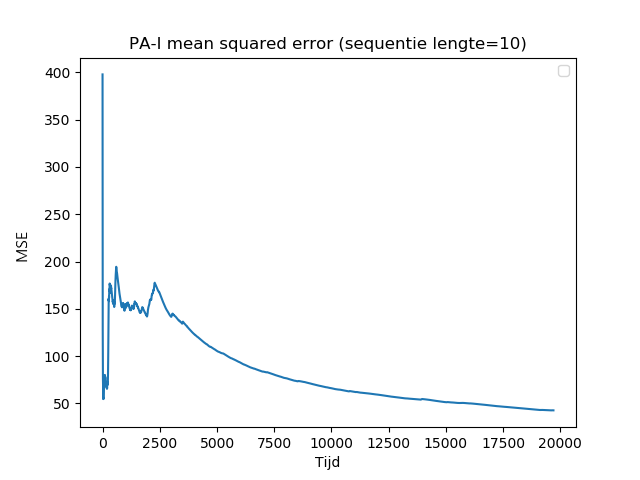
\includegraphics[width=\linewidth]{images/evaluatie/seqlen10.png}
\end{subfigure}
\begin{subfigure}{.49\textwidth}
  \centering
  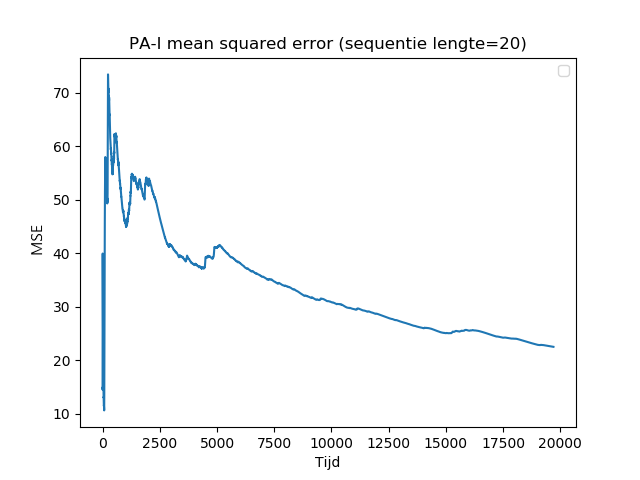
\includegraphics[width=\linewidth]{images/evaluatie/seqlen20.png}
\end{subfigure}
\begin{subfigure}{.49\textwidth}
  \centering
  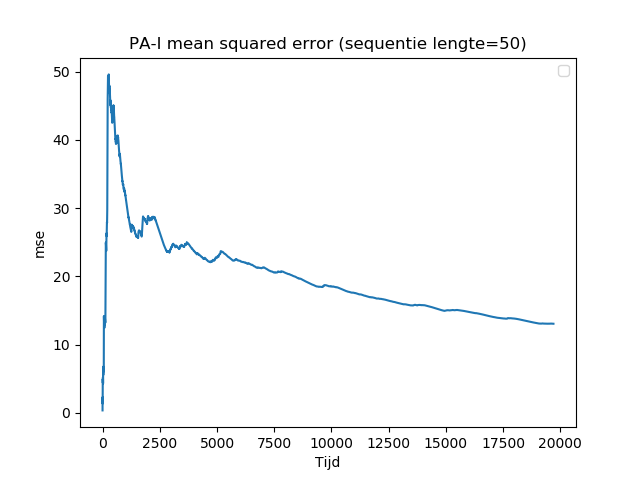
\includegraphics[width=\linewidth]{images/evaluatie/seqlen50.png} 
\end{subfigure}
\begin{subfigure}{.49\textwidth}
  \centering
  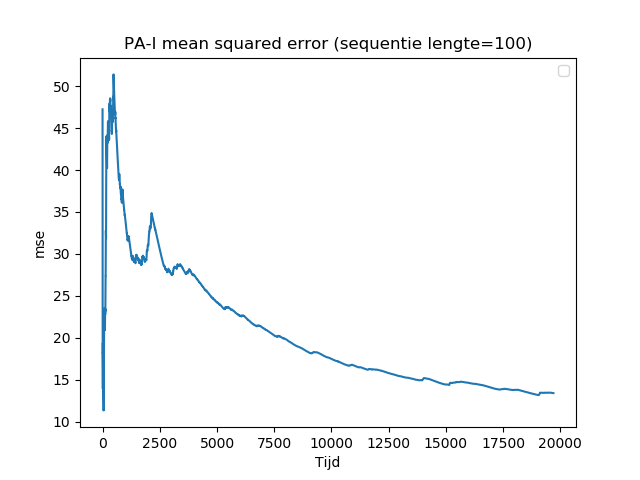
\includegraphics[width=\linewidth]{images/evaluatie/seqlen100.png}   
\end{subfigure}
\caption{De invloed van sequentielengte op de error}
\label{fig:seqlen error}
\end{figure}
\section{Algoritmes}
\subsection{Passive Aggressive Algorithm}
Er zijn enkele hyperparameters die ingesteld kunnen worden. $Max\_ iter$ is het maximum aantal iteraties dat het algoritme probeert bij te leren. Tol is een parameter die bepaalt of het algoritme vroegtijdig stopt. Dit gebeurt wanneer de fout na een leercyclus met minder dan tol verbeterd. In de testomgeving, met $max\_ iter=25$ en $tol=0.1$, wordt deze vroegtijdige stop altijd behaalt. Met andere woorden, na 25 iteraties heeft het algoritme de trainingsdata geleerd.
\\\\
Een laatste interessante parameter is C: de agressiviteit parameter. Hoe hoger deze is, hoe agressiever het algoritme de gewichten gaat bijwerken. De onderstaande figuur toont hoe de C parameter de mean squared error beïnvloed van zowel PA-I als PA-II. C is de enige parameter die aangepast wordt.
\\\\
Bijna alle tests convergeren naar een mse tussen tien en vijftien, met een gemiddelde tussen dertien en veertien. Wat het verschil is tussen PA-I en PA-II valt niet duidelijk te zien. In de paper van Crammer et al. \cite{pa algorithm} worden beide versies vergeleken op basis van instance noise en label noise. In beide gevallen scoren PA-I en PA-II aanzienlijk beter dan het standaard algoritme. In dit experiment scoren PA-I en PA-II gelijkaardig.
\\\\
Figuur \ref{fig:gemiddeld aantal keer trainen pa} toont de invloed van C op het aantal keer trainen. Het verschil tussen de verschillende settings is klein. De “stappen” die genomen worden tijdens het trainen zullen dus vaak klein genoeg zijn zodat C=1 agressief genoeg is. Het is dus niet nodig om hoge C-waarden (5-10) te gebruiken. Deze data is genomen over tien sessies, van elk 20000 iteraties, en duurde telkens gemiddeld 90 seconden. 
\\\\
\begin{figure}[h]
	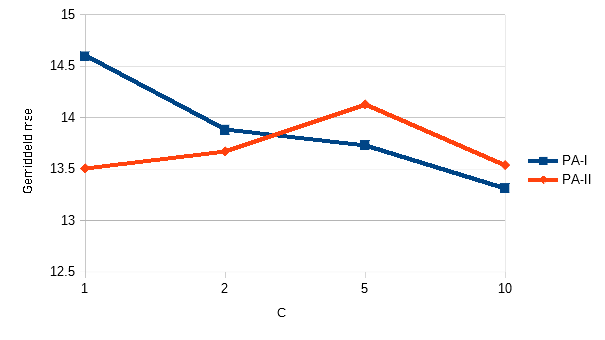
\includegraphics[width=\linewidth]{images/evaluatie/gemiddeldmsepa.png}
	\caption{De invloed van C op mse van PA}
	\label{fig:invloed C op PA}
\end{figure}
\newpage
\begin{figure}[t]
	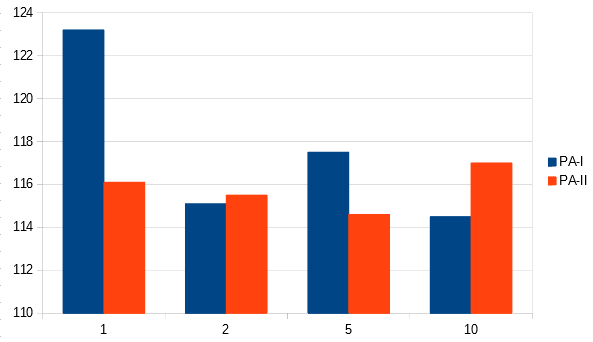
\includegraphics[width=\linewidth]{images/evaluatie/aantalkeertrainenpa.png}
	\caption{Gemiddeld aantal keer trainen PA}
	\label{fig:gemiddeld aantal keer trainen pa}
\end{figure}
\subsection{Decision Tree en Random Forest}
De belangrijkste parameter bij deze rule-based learners is de $max\_ depth$. Dit is een moeilijk in te schatten parameter, vooral voor de DT. Diepere DT’s maken betere voorspellingen, maar op een bepaald punt begint de DT te overfitten. Bij RF kan ook het aantal bomen ingesteld worden. Hoe meer bomen er gebruikt worden, hoe minder invloed ruis heeft op voorspellingen en hoe beter de voorspellingen worden.
\\\\
DT’s en RF’s convergeren beide naar ongeveer dezelfde mean squared error. Diepere bomen leiden evident naar een lagere mean squared error. Algemeen zijn grotere RF’s beter, maar in deze situatie is het verschil klein.
\\\\
Voor DT, daalt het gemiddeld aantal trainingen spectaculair tussen diepte drie en vier (figuur \ref{fig:invloed diepte en aantal bomen trainen}). Een DT van diepte drie zal dus geen goede oplossing zijn. RF’s daarentegen presteren wel goed met een diepte van drie. Een DT/RF dieper dan vier is niet nodig, aangezien dit geen groot voordeel oplevert en mogelijk overfit.
\\\\
De uitvoeringstijd (figuur \ref{fig:invloed diepte en aantal bomen uitvoeringstijd}) lijkt geen probleem te vormen voor grotere RF. Het verschil tussen de uitvoeringstijden van een RF met diepte drie en de andere is te wijten aan het aantal keer dat getraind moest worden op diepte drie.

\begin{figure}[t!]
\centering
\begin{subfigure}{\textwidth}
  \centering
    \hspace*{-0.75cm}                                                           
  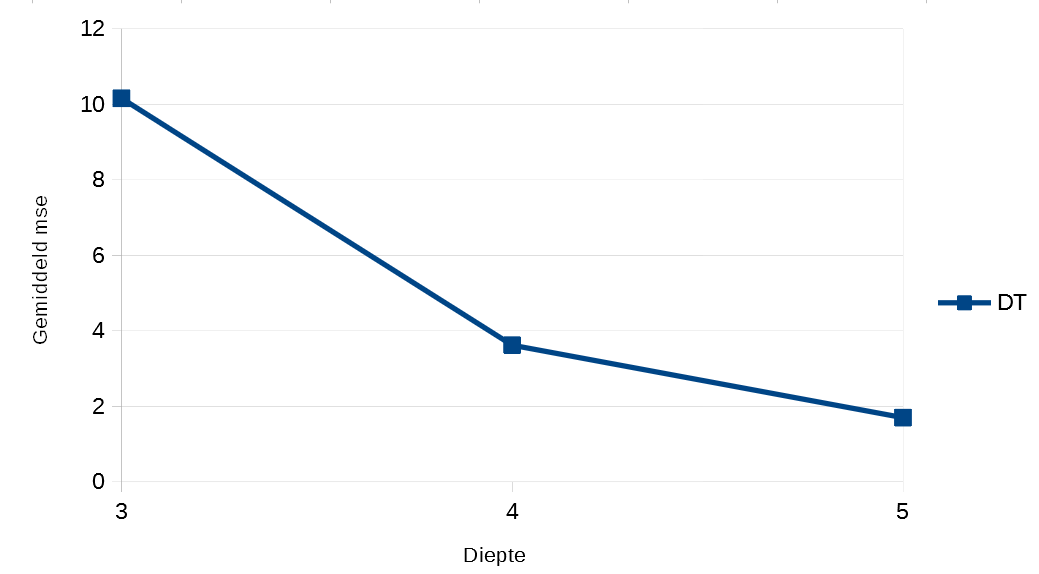
\includegraphics[width=\linewidth]{images/evaluatie/gemiddeldmsedt.png}
\end{subfigure}
\begin{subfigure}{\textwidth}
  \centering
  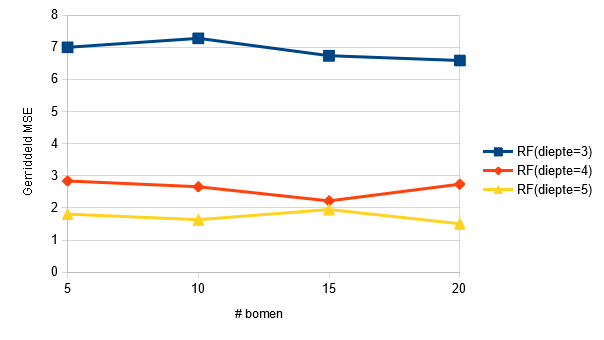
\includegraphics[width=\linewidth]{images/evaluatie/gemiddeldmserf.png}
\end{subfigure}
\caption{De invloed van diepte en aantal bomen op de gemiddelde mean squared error van DT en RF (10 keer 20 iteraties)}
\label{fig:invloed diepte en aantal bomen mse}
\end{figure}
\begin{figure}[t!]
\centering
\begin{subfigure}{\textwidth}
  \centering
    \hspace*{-0.75cm}                                                           
  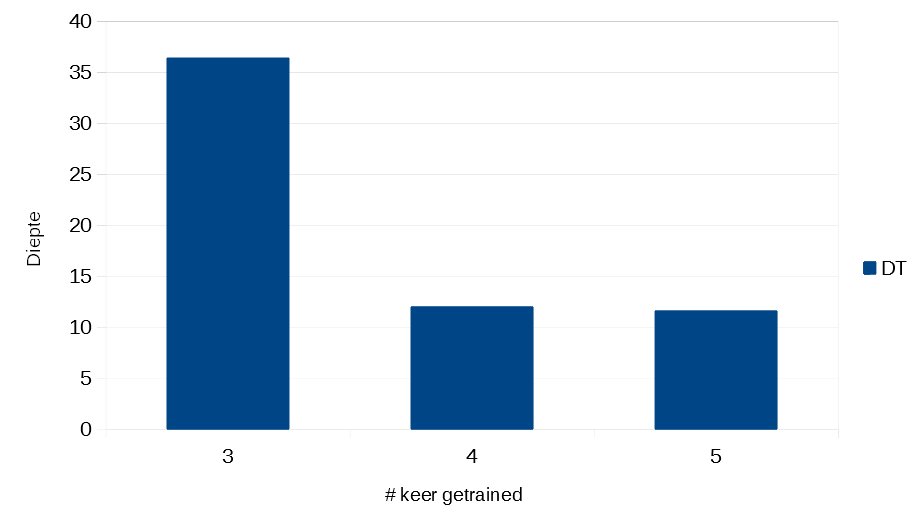
\includegraphics[width=\linewidth]{images/evaluatie/aantalkeertrainendt.png}
\end{subfigure}
\begin{subfigure}{\textwidth}
  \centering
  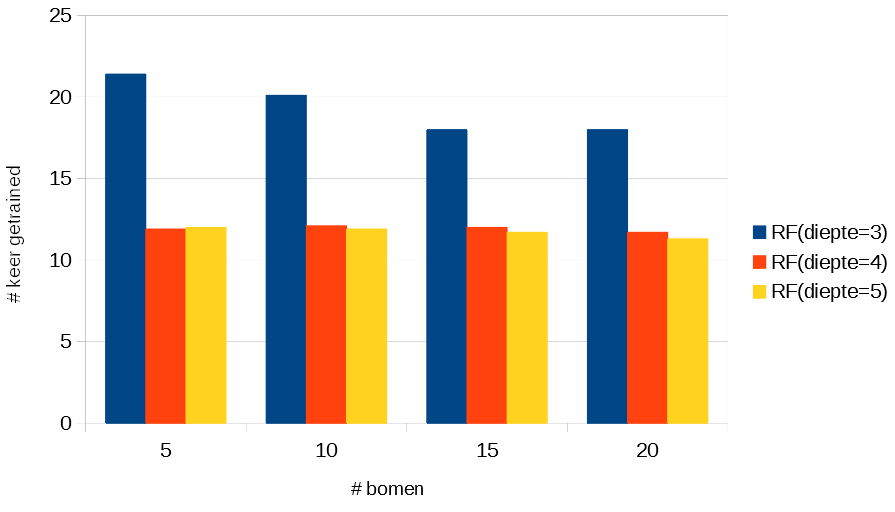
\includegraphics[width=\linewidth]{images/evaluatie/aantalkeertrainenrf.png}
\end{subfigure}
\caption{De invloed van diepte en aantal bomen op het gemiddeld aantal keer trainen van DT en RF (10 keer 20 iteraties)}
\label{fig:invloed diepte en aantal bomen trainen}
\end{figure}
\begin{figure}[t!]
\centering
\begin{subfigure}{\textwidth}
  \centering
  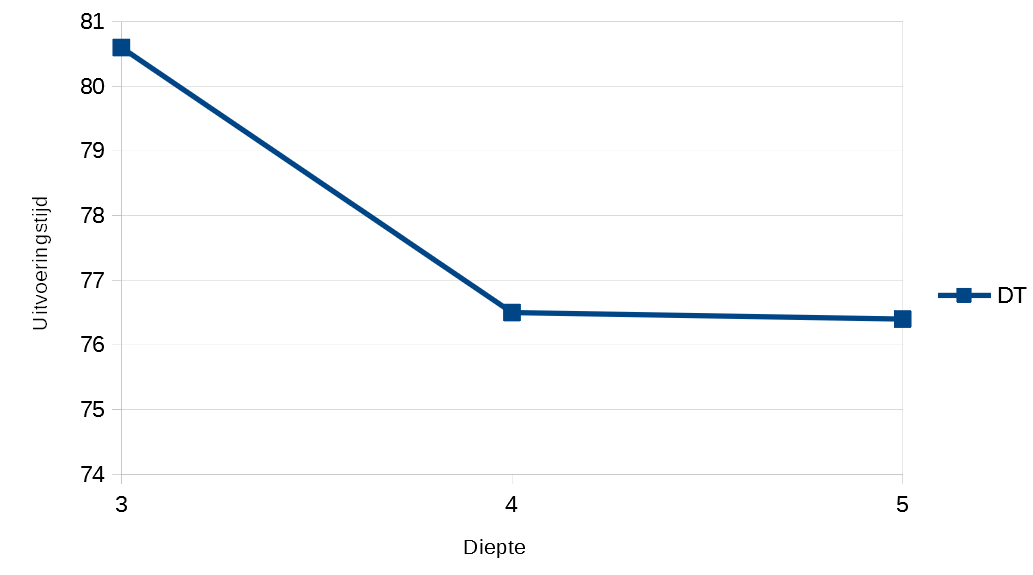
\includegraphics[width=\linewidth]{images/evaluatie/uitvoeringstijddt.png}
\end{subfigure}
\begin{subfigure}{\textwidth}
  \centering
  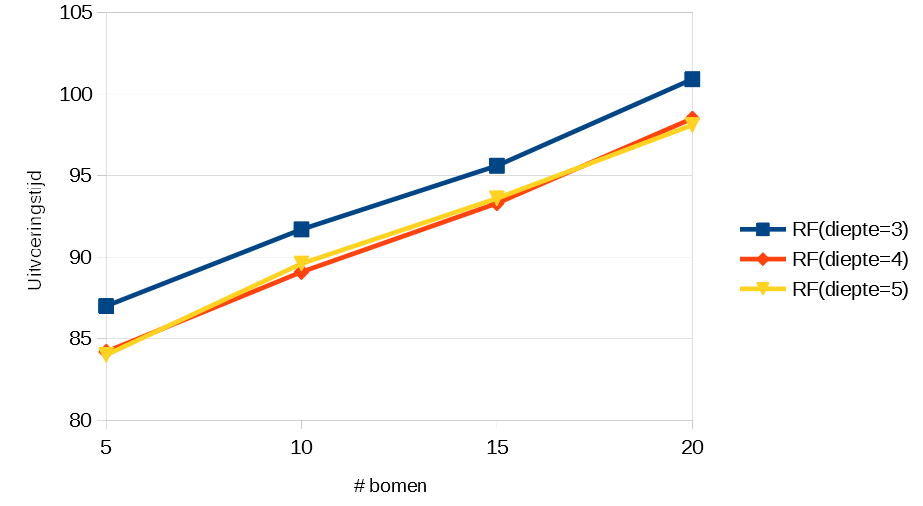
\includegraphics[width=\linewidth]{images/evaluatie/uitvoeringstijdrf.png}
\end{subfigure}
\caption{De invloed van diepte en aantal bomen op de uitvoeringstijd van DT en RF (10 keer 20 iteraties)}
\label{fig:invloed diepte en aantal bomen uitvoeringstijd}
\end{figure}
